\section{Numerical Verification}
\label{sec:numerical-verification}

This section reports implementation and numerical-verification evidence for
the selected solver. The checks below address reproducibility, descriptor
health, numerical consistency, and emitted data contracts. They do not become
clinical validation, pressure or FFR accuracy evidence, full transient FEM
validation, or scientific equivalence beyond the metrics actually compared.

\subsection{Software and Descriptor Checks}
\label{subsec:verification-reproducibility}
\label{subsec:package-benchmark-suite}

The implementation includes an internally reproducible benchmark pipeline for
the Julia solver and Python CLI. The suite records
descriptor health, sampled self-convergence, native/SciML cross-integrator
discrepancy, stationary-Stokes projection checks, rheology/profile sensitivity,
OpenBF-style boundary handling, resolved-velocity diagnostics, and Python
CPU/MPS checks for the emitted CSV records.

\begin{lstlisting}[basicstyle=\ttfamily\footnotesize,breaklines=true]
./scripts/julia-release simulations/run_package_benchmark.jl \
  --profile overnight \
  --output-dir simulations/output/package_benchmark/<run_id> \
  --overwrite \
  --include-python \
  --include-resolved3d \
  --publish-report-assets

pipenv run python scripts/render_package_benchmark_figures.py \
  --benchmark-dir simulations/output/package_benchmark/<run_id>
\end{lstlisting}

The smoke profile is a deterministic wiring check. The overnight profile
expands the same schemas to the descriptor-health, refinement, native/SciML
cross-integrator, stationary-Stokes projection, rheology/profile, OpenBF-style
boundary, resolved-velocity, and Python CPU/Torch-MPS comparison stages.
Optional SciPy and resolved-3D inputs are treated as availability boundaries:
absent inputs produce structured skipped rows rather than manuscript claims.

\IfFileExists{figures/static/static/tables/package-benchmark/package-benchmark-summary.tex}{%
    \begin{table}[!htb]
    \centering
    \scriptsize
    \caption{Benchmark stage summary.}
    \begin{tabular}{@{}lrrr@{}}
        \toprule
        Stage & Rows & OK & Skipped/error \\
        \midrule
        case results & 18 & 18 & 0 \\
        refinement & 128 & 128 & 0 \\
        backend parity & 18 & 18 & 0 \\
        stokes ic & 12 & 12 & 0 \\
        rheology profile & 60 & 60 & 0 \\
        boundary openbf & 3 & 3 & 0 \\
        resolved3d & 4 & 4 & 0 \\
        \bottomrule
    \end{tabular}
\end{table}

}{%
    \begin{center}
    \small
    \emph{Benchmark table fragment unavailable in this checkout. Run
    the benchmark renderer to populate
    \path{figures/static/static/tables/package-benchmark/}.}
    \end{center}
}

\subsection{Boundary Diagnostics}
\label{subsec:boundary-diagnostics}

OpenBF-style boundary rows and the emitted comparison records check that the
selected inlet, outlet, and descriptor conventions remain machine-readable.
For the resolved-velocity comparison, the archived rows include accepted step
counts, minimum area, maximum speed, pressure extrema, section counts, minimum
intersection counts, $\alpha_{\mathrm{eff}}$ extrema, and the minimum
characteristic radicand for the final sampled state. The archived
cross-model runs used here did not persist positivity-activation counts, total
projected correction, realized CFL range, mass-balance defect, or backend
tolerances for the comparison artifact; these quantities are verification
limitations rather than evidence.

\subsection{Sampled Self-Convergence}
\label{subsec:sampled-self-convergence}

\begin{figure}[H]
    \centering
    \IfFileExists{figures/static/static/rendered/package-benchmark-convergence.pdf}{%
        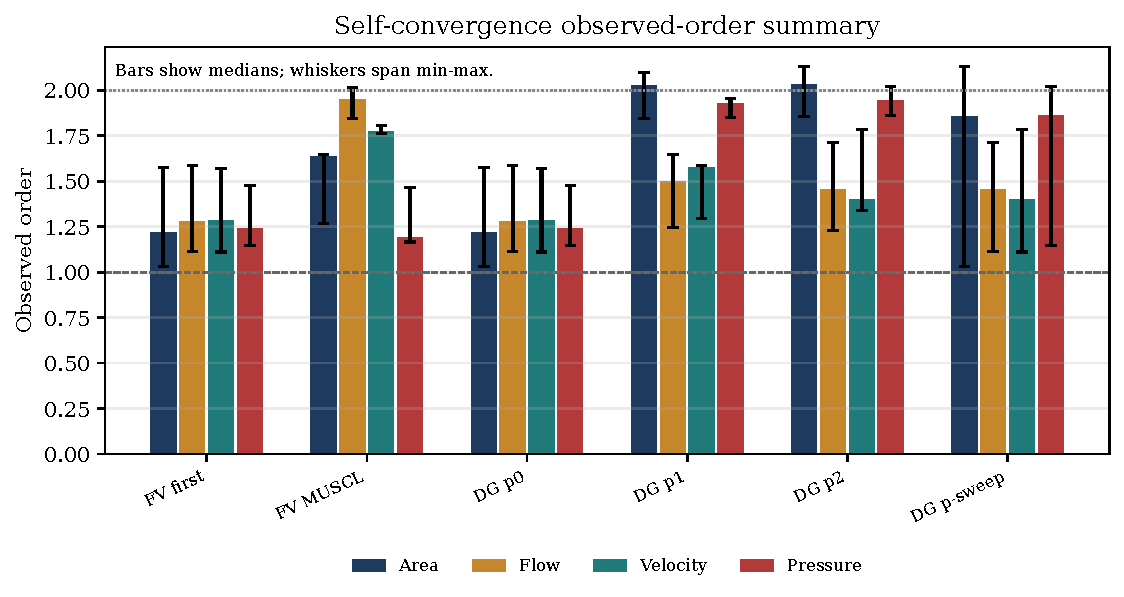
\includegraphics[width=0.95\linewidth]{figures/static/static/rendered/package-benchmark-convergence.pdf}
    }{%
        \fbox{\parbox{0.86\linewidth}{\centering Benchmark convergence
        asset unavailable in this checkout.}}
    }
    \caption{Self-convergence observed-order summary emitted by the
    benchmark renderer. Bars report median observed order by method and metric;
    whiskers show the observed min--max range across the benchmarked
    refinements. DG bars are implementation diagnostics emitted by the
    benchmark suite; Appendix~\ref{app:num-current-solver-operator} specifies
    the finite-volume operator used for the reported comparison. This is an
    internal convergence diagnostic, not external validation evidence.}
    \label{fig:package-benchmark-convergence}
\end{figure}

\subsection{Cross-Integrator Discrepancies}
\label{subsec:cross-integrator-discrepancies}

\begin{figure}[H]
    \centering
    \IfFileExists{figures/static/static/rendered/package-benchmark-backend-parity.pdf}{%
        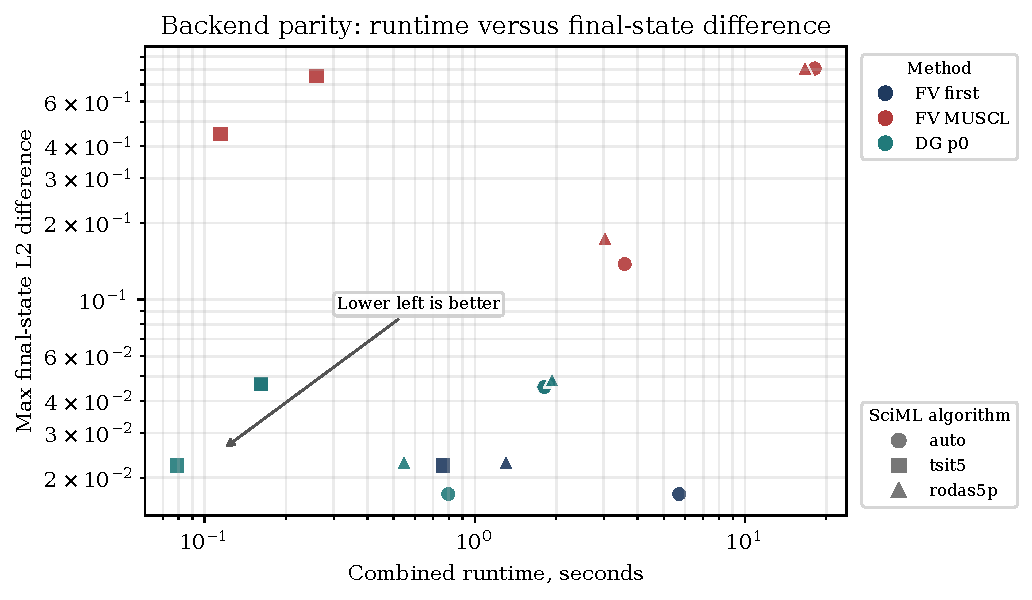
\includegraphics[width=0.95\linewidth]{figures/static/static/rendered/package-benchmark-backend-parity.pdf}
    }{%
        \fbox{\parbox{0.86\linewidth}{\centering Benchmark
        cross-integrator discrepancy asset unavailable in this checkout.}}
    }
    \caption{Native/SciML cross-integrator discrepancy versus runtime for
    benchmarked compatible methods. Color identifies the method family and
    marker shape identifies the SciML algorithm. The plotted scalar is the
    maximum of emitted componentwise L2 difference columns, so it is a software
    diagnostic rather than a dimensionally homogeneous physical norm.}
    \label{fig:package-benchmark-backend-parity}
\end{figure}

\subsection{Stationary-Stokes Projection Checks}
\label{subsec:stationary-stokes-projection-checks}

The stationary-Stokes projection checks are included as implementation
diagnostics for the local resolved-flow pipeline. They check that the
projection and report assets are emitted under a reproducible schema. They do
not constitute transient 3D validation of the 1D solver.

\begin{figure}[!htb]
    \centering
    \IfFileExists{figures/static/static/rendered/package-benchmark-resolved3d.pdf}{%
        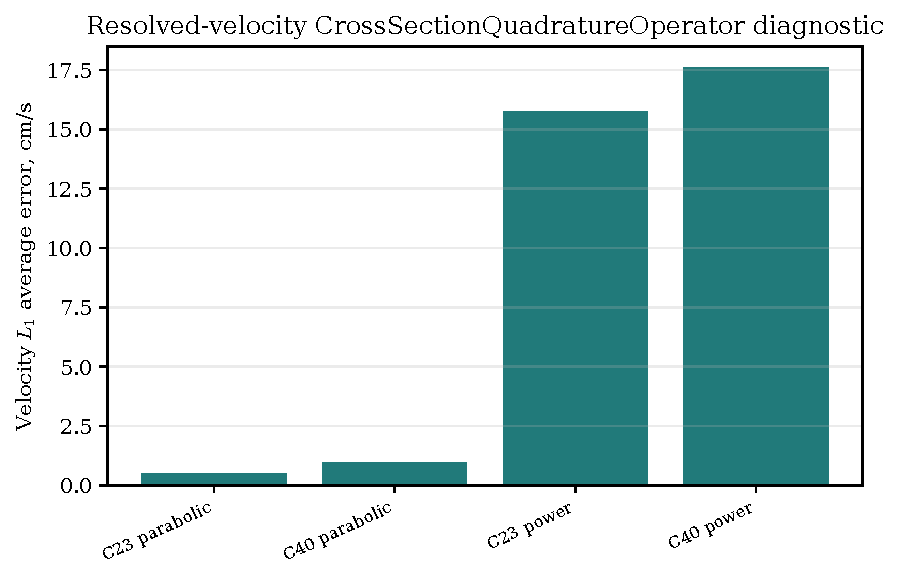
\includegraphics[width=0.74\linewidth]{figures/static/static/rendered/package-benchmark-resolved3d.pdf}
    }{%
        \fbox{\parbox{0.86\linewidth}{\centering Benchmark
        resolved-velocity diagnostic asset unavailable in this checkout.}}
    }
    \caption{Resolved-velocity output-operator diagnostic summary for the
    available local cases. The rendered value is the section-wise velocity
    mean absolute discrepancy for the declared
    \texttt{CrossSectionQuadratureOperator}.}
    \label{fig:package-benchmark-resolved3d}
\end{figure}

\subsection{Verification Summary}
\label{subsec:verification-summary}

\begin{figure}[H]
    \centering
    \IfFileExists{figures/static/static/rendered/package-benchmark-rheology-profile.pdf}{%
        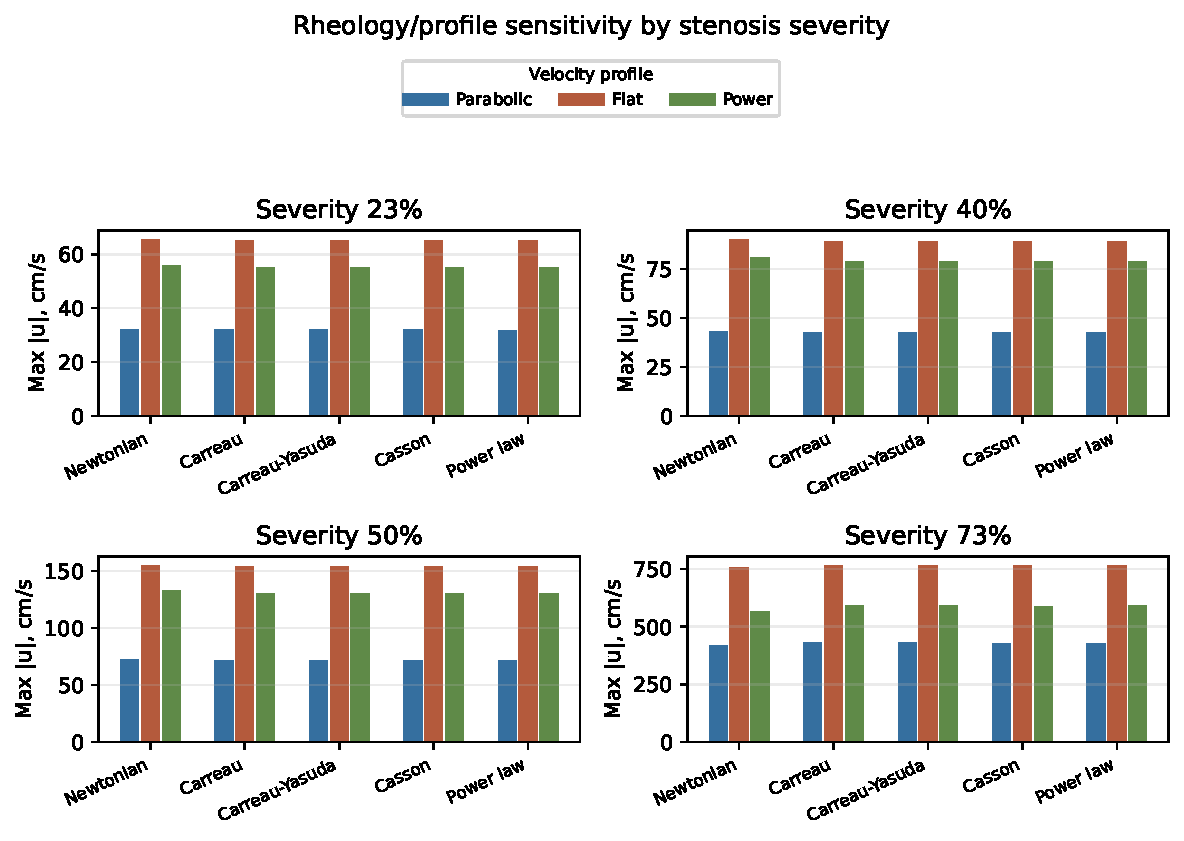
\includegraphics[width=0.95\linewidth]{figures/static/static/rendered/package-benchmark-rheology-profile.pdf}
    }{%
        \fbox{\parbox{0.86\linewidth}{\centering Benchmark
        rheology/profile asset unavailable in this checkout.}}
    }
    \caption{Rheology/profile sensitivity summary for declared descriptor
    combinations. Facets separate stenosis severity; grouped bars separate the
    rheology and velocity-profile descriptors. The diagnostic shows how the
    maximum speed responds to descriptor choices within the emitted benchmark
    records.}
    \label{fig:package-benchmark-rheology-profile}
\end{figure}

\begin{figure}[!htb]
    \centering
    \IfFileExists{figures/static/static/rendered/package-benchmark-python-mps.pdf}{%
        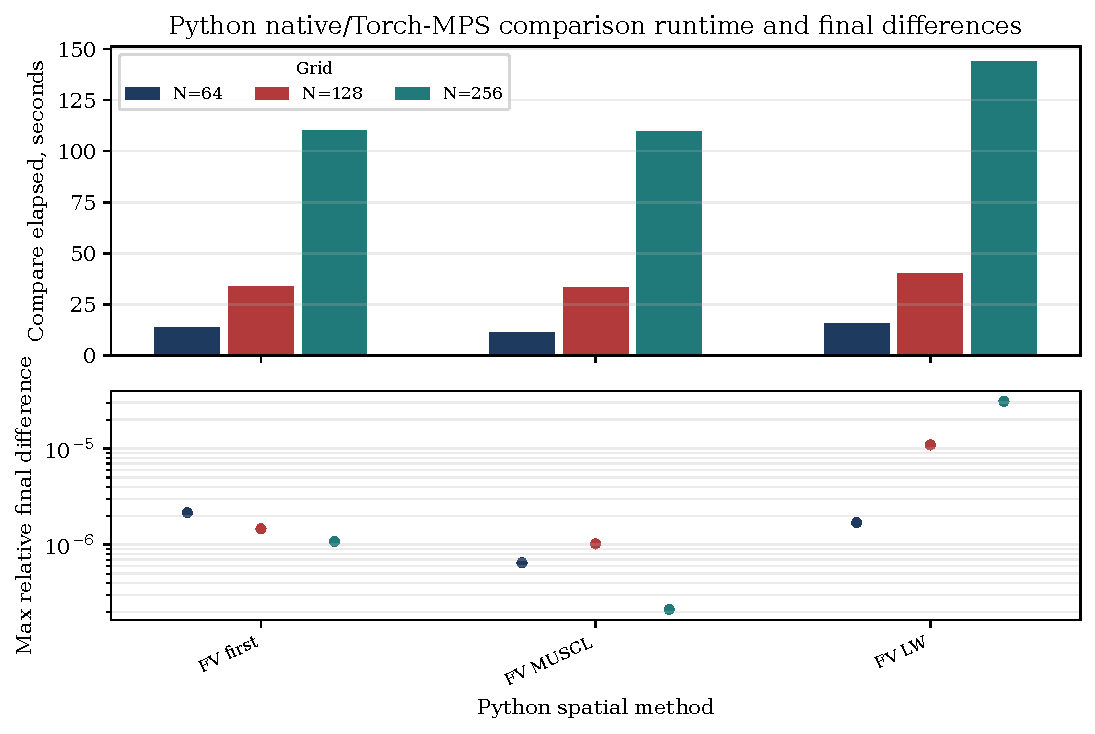
\includegraphics[width=0.95\linewidth]{figures/static/static/rendered/package-benchmark-python-mps.pdf}
    }{%
        \fbox{\parbox{0.86\linewidth}{\centering Python/MPS benchmark asset
        unavailable in this checkout.}}
    }
    \caption{Python native CPU versus Torch-MPS comparison for the Python CLI
    surface. The top panel reports elapsed time by method and grid size; the
    lower panel reports the maximum relative final-state difference across the
    emitted area and flow summaries.}
    \label{fig:package-benchmark-python-mps}
\end{figure}

The verification record supports the reported finite-volume /
time-integration workflow and data contracts. It does not yet persist every
quantity needed for a stronger verification claim, including positivity
activation counts, total projection correction, realized CFL extrema,
mass-balance defect, and comparison-run backend tolerances.

\FloatBarrier
